\section{Vector Field Visualisation}
\begin{itemize}
\item A \emph{static vector field} $v(x)$ is a vector-valued function of space.
\item A \emph{time-dependent vector field} $v(x,t)$ also depends on time.
\end{itemize}
In the case of \emph{velocity fields}, the terms \emph{steady} and \emph{unsteady flow} are used. 

The dimensions of $ x$ and $ v$ are equal, often $2$ or $3$ and we denoted the components by $x,\ y,\ z$ and $u,\ v,\ w$:
    \begin{align*}
         x = (x,\ y,\ z),\qquad v =(u,\ v,\ w).
    \end{align*}
Sometimes a vector field is defined on a surface $x(i,j)$. The vector field is then a function of parameters and time:
    \begin{align*}
        v(i,j,t).
    \end{align*}

\subsection{Visualisation}
An elementary visualisation of a vector field is to \emph{draw arrows}:
\begin{itemize}
    \item At the data points (gird nodes or cell centers), or
    \item at a new (uniform) grids. For 3D fields it's often a 2D slice.
\end{itemize}

Arrows can visualise:
\begin{itemize}
    \item Direction
    \item Relative magnitude (when appropriately scaled(
    \item Time dependency (when animated)
\end{itemize}

\paragraph{Problems} $\ $
\begin{itemize}
    \item It is not clear whether arrows represent vector values at the start point or at the midpoint of the arrow.
    \item Of there exist no satisfactory scaling factors:
        \begin{itemize}
            \item Large scaling: Arrows occlude each other
            \item Small scaling: Direction is not recognisable in some regions
            \item Fixed length: Magnitued information is lost.
        \end{itemize}
\end{itemize}

\subsection{Vector fields as ODEs}
For simplicity, the vector field is now interpreted as \emph{velocity field}. The field $v(x,t)$ describes the connection between location and velocity of a (massless) particle. Which can equivalently be expressed as an \emph{ordinary differential equation}:
\begin{align*}
    \dot x(t) = v(x(t),t).
\end{align*}
This ODE, together with an \emph{initial condition} 
\begin{align*}
    x(t_0) = x_0,
\end{align*}
is a so-called \emph{initial value problem} (IVP). Its solution is the \emph{integral curve} (or \emph{trajectory})
\begin{align*}
    x(t) = x_0 + \int_{t_0}^t v(x(\tau),\tau)d\tau.
\end{align*}

The integral curve is a \emph{pathline} decribing the \emph{path} of a massless \emph{particle} which was released at time $t_0$ at position $x_0$.

Remark: $t<t_0$ is allowed.

For static fields the ODE is \emph{autonomous}:
\begin{align*}
    \dot x (t) = v(x(t))
\end{align*}
and its integral curves
\begin{align*}
    x(t) = x_0 + \int_{t_0}^t v(x(\tau)) d\tau
\end{align*}
are called \emph{field lines} or in the case of velocity fields \emph{streamlines}.

\begin{itemize}
    \item In \emph{static vector fields} pathlines and streamlines are \emph{identical}.
    \item In \emph{time-dependent} vector fields \emph{instantaneous streamlines} can be computed from a "snapshot" at a fixed time $T$ (which is a static vector field):
    \begin{align*}
        v_T (x) = v(x,T).
    \end{align*}
\end{itemize}
In practice time-dependent fields are often given as a dataset per time step. Each dataset is then a snapshot.


Computing streaklines or timelines is more expensive than solving a single IVP.

\subsubsection{Pathlines}
Pathlines are the trajectories that individual fluid particles follow. These can be thought of as "recording" the path of a fluid element in the flow over a certain period. The direction the path takes will be determined by the streamlines of the fluid at each moment in time.\footnote{\url{https://en.wikipedia.org/wiki/Streamlines,_streaklines,_and_pathlines}}

\begin{itemize}
    \item Are physically meaningful
    \item Allow comparison with experiment (observe marked particles)
    \item Are well suited for dynamic visualisation (of particles).
\end{itemize}


\subsubsection{Streamlines}
Streamlines are a family of curves that are instantaneously tangent to the velocity vector of the flow. These show the direction a fluid element will travel in at any point in time.\footnote{\url{https://en.wikipedia.org/wiki/Streamlines,_streaklines,_and_pathlines}}
\begin{itemize}
    \item Are only geometrically but not physically meaningful,
    \item Are easiest to compute (no temporal interpolation, single IVP),
    \item Are better suited for static visualisation (prints),
    \item Don't intersect (under reasonable assumptions)
\end{itemize}

\paragraph{Inputs} $\ $
\begin{itemize}
    \item Static vector field $v(x)$
    \item Seed points with time of release $(x_0, t_0)$
    \item Control Parameters:
        \begin{itemize}
            \item Step size (temporal, spatial or in local coordinates)
            \item Step count limit, time limit, etc...
            \item Order of integration scheme
        \end{itemize}
\end{itemize}
\paragraph{Output} Streamlines as "polylines", with possible attributes.

\paragraph{Preprocessing} $\ $
\begin{itemize}
    \item Set up search structure for point location
    \item For each seed point:
        \begin{itemize}
            \item \emph{Global point location}: \\ Given a point $x$, find the cell containing $x$ and the local coordinates $(\xi, \nu, \zeta)$. \\
            Alternatively if the grid is structured find the computational space coordinates
            \begin{align*}    
                (i+\xi, j+\nu, k+\zeta)
            \end{align*}
            \item If $x$ is not found in a cell then remove the seed point.
        \end{itemize}
        
\end{itemize}
\paragraph{Integration} For each seed point $x$:
\begin{itemize}
\item Interpolate $v$ trilinearly to local coordinates $(\xi, \nu, \zeta)$
\item Do an integration step producing a new point $x'$
\item \emph{Incremental point location}: For position $x'$ find cell and local coordinates $(\xi', \nu', \zeta')$ making use of information (coordinates, local coordinates, cell) of old point $x$.
\end{itemize}
\paragraph{Integration step} Widely used methods:
\begin{itemize}
    \item \emph{Euler}, inaccurate, used only in special speed-optimised techniques:
        \begin{align*}
            x_\text{new} = x+ v(x,t)\cdot \Delta t
        \end{align*}
    \item \emph{Runga-Kutta}, $2^{nd}$ or $4^{th}$ order.  Higher order schemes are often too slow for visualisation. Yeung/Pope 1987 showed that when using standard trilinear interpolation \emph{interpolation errors} dominate \emph{integration errors}.
    \item There are several options for choosing a step size:
        \begin{itemize}
            \item Fixed time stepping $\Delta t$
            \item Fixed spatial step $\Delta s$:
                
                The time step is derive from he spatial step
                    \begin{align*}
                        \Delta t = {\Delta s \over \norm{v(x)}}
                    \end{align*}
                which needs to be corrected iteratively and is used for methods such as LIC.
            \item Adaptive:
                \begin{itemize}
                    \item Adapting to grid resolution (such as cell size)
                    \item Adapting to data variation (Runge-Kutta-Fehlberg method)
                    \item Used for interactive viewing (with zooming)
                \end{itemize}
            \end{itemize}
        
\end{itemize}


\paragraph{Termination criteria} $\ $
\begin{itemize}
    \item Grid boundary reached
    \item Step count limit reached
    \item Optional: Velocity close to zero
    \item Optional: Time limit reached
    \item Optional: Arc length limit reached
\end{itemize}


\subsubsection{Streaklines}
Streaklines are the locus of points of all the fluid particles that have passed continuously through a particular spatial point in the past. Dye steadily injected into the fluid at a fixed point extends along a streakline.

\begin{itemize}
    \item Are physically meaningful
    \item Allow a direct comparison with the experiment (i.e. dye injection)
    \item Are well suited for static and dynamic visualisation
    \item Are a good choice for fast moing vortices
    \item Can be approximated by a set of disconnected particles.
\end{itemize}


Algorithm:
\begin{enumerate}
    \item For time samples $t_0$, $t_1$, $\ldots$, $t_n$ solve the IVP
        \begin{align*}
            \dot x_i (t) &= v(x_i(t), t)\\
             x_i(t_i) &= y
        \end{align*}
    \item Extract the point $x_i(t_n))$
\end{enumerate}

In numerical computation the temporal interval must be \emph{adaptively refined} if two successive particles diverge too much.

\subsubsection{Timelines}
Timelines are the lines formed by a set of fluid particles that were marked at a previous instant in time, creating a line or a curve that is displaced in time as the particles move.


\begin{itemize}
    \item Are physically meaningful
    \item Are well suited for static and dynamic visualisation
    \item Can be approximated by a set of disconnected particles.
\end{itemize}



Algorithm:
\begin{enumerate}
    \item For point samples $y_0$, $y_1$, $\ldots$, $y_n$ on the seed curve solve the IVP:
        \begin{align*}
            \dot x_i (t) &= v(x_i(t),t)\\
            x_i(t_0) = y_i
        \end{align*}
    \item From the integral curve $x_i(t)$ extract the point $x_i(T)$.
    \item Connect these points.
\end{enumerate}
The result is a timeline for time $T$.

In the numerical computation the spatial interval must be \emph{adaptively refined} if two neighbour particles diverge too much.


\subsection{The Stencil Walk algorithm}
Computing the \emph{incremental point location} is nontrivial for curvilinear and unstructured grids.

Buning's \emph{stencil walk} algorithm solves this provlem.

\paragraph{Given}$\ $
\begin{itemize}
    \item Point with coordinates $x$
    \item Cell (as three parameters $(i,j,k)$ or as index $c$ respectively)
    \item Local coordinates $(\xi, \nu, \zeta)$
    \item Coordinates of a new point $x'$
\end{itemize}
\paragraph{Wanted} $\ $
\begin{itemize}
    \item New cell as $(i',j', k')$ or as index $c'$ respectively
    \item New local coordinates $(\xi, \nu, \zeta)$
\end{itemize}

\paragraph{Algorithm}
In a first phase the algorithm find the cell containing $x'$ by iteratively doing:
\begin{itemize}
    \item Take the difference vector $\Delta x = x'-x$
    \item Intersecting the ray $x+t \Delta x$ with the cell boundary giving a $t$ value.
        \begin{itemize}
            \item Linearise the coordinate transform 
                \begin{align*}
                    \phi: (\xi, \nu, \zeta)\mapsto (x,y,z)
                \end{align*}
                in the point $x=(x,y,z)$ by computing the \emph{Jacobian}
                \begin{align*}
                    J={\delta (x,y,z)\over \delta (\xi, \nu, \zeta)} = 
                        \left[
                            {\delta \phi\over \delta \xi} | {\delta \phi\over \delta \nu} | {\delta \phi\over \delta \zeta}
                        \right].
                \end{align*}
            \item Using the \emph{Jacobian} to transform the difference vector $\Delta x = x'-x$ into the local coordinate frame of the cell:
                \begin{align*}
                    (\Delta \xi, \Delta \nu, \Delta \zeta) = J^{-1} \Delta x.
                \end{align*}
            \item Find the intersection of the ray
                \begin{align*}
                    (\xi, \nu, \zeta) + t(\Delta \xi, \Delta \nu, \Delta \zeta)
                \end{align*}
                with the cell boundary having the equations:
                    \begin{align}
                         \xi, \nu, \zeta &= 0\\
                         \xi, \nu, \zeta &= 1 &\text{for hex cell}\\
                         \xi + \nu + \zeta &= 1 &\text{for tet cell}\\
                         0 \leq \xi, \nu, \zeta &\geq 1 &\text{inequalities}
                    \end{align}

        \end{itemize}
        Due to linearisation the point is not exact and in most cases the correct neighbour cell is found.
    \item If $t\geq 1$ the point $x'$ lies in the current cell and iteration can be stopped.
    \item Otherwise move to the neighbour cell adjacent at the intersection point
    \item If no such cell exists terminate with failure
    \item Set the \emph{cell centroid} as the new $x$ for the next iteration.
\end{itemize}


\subsubsection{Problems}
If the cells are sufficiently skewed the algorithm can walk away from the target cell.
\begin{figure}[H]
    \centering
    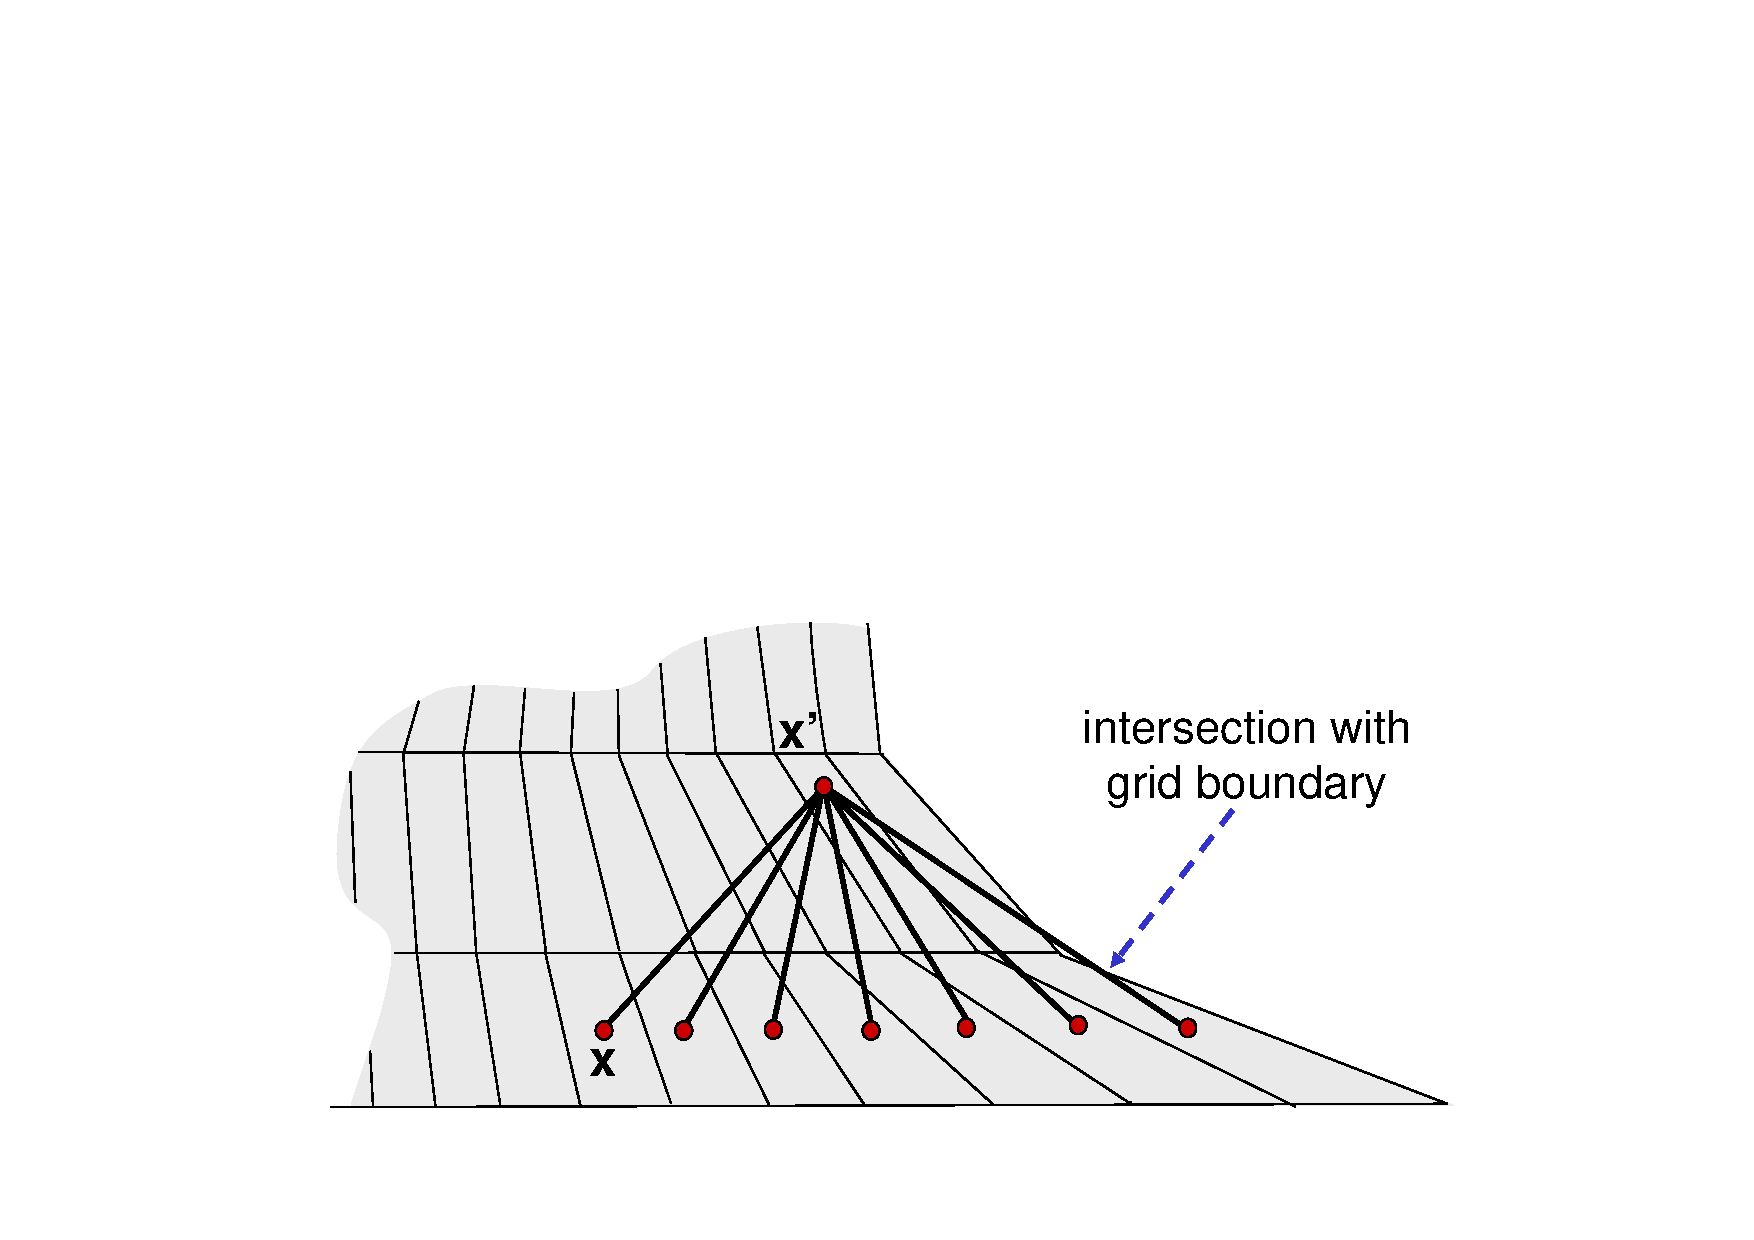
\includegraphics[width=0.8\textwidth]{img/05_stencil_walk_problems}
\end{figure}

This problem can be solved with a \emph{modification} of the algorithm:
\begin{itemize}
    \item Keep ray $(x,x')$ unchanged
    \item New Problem: Cell faces of the type \emph{quadrangle} (nonplanar!) can be intersected \emph{twice}!
    \begin{figure}[H]
    \centering
    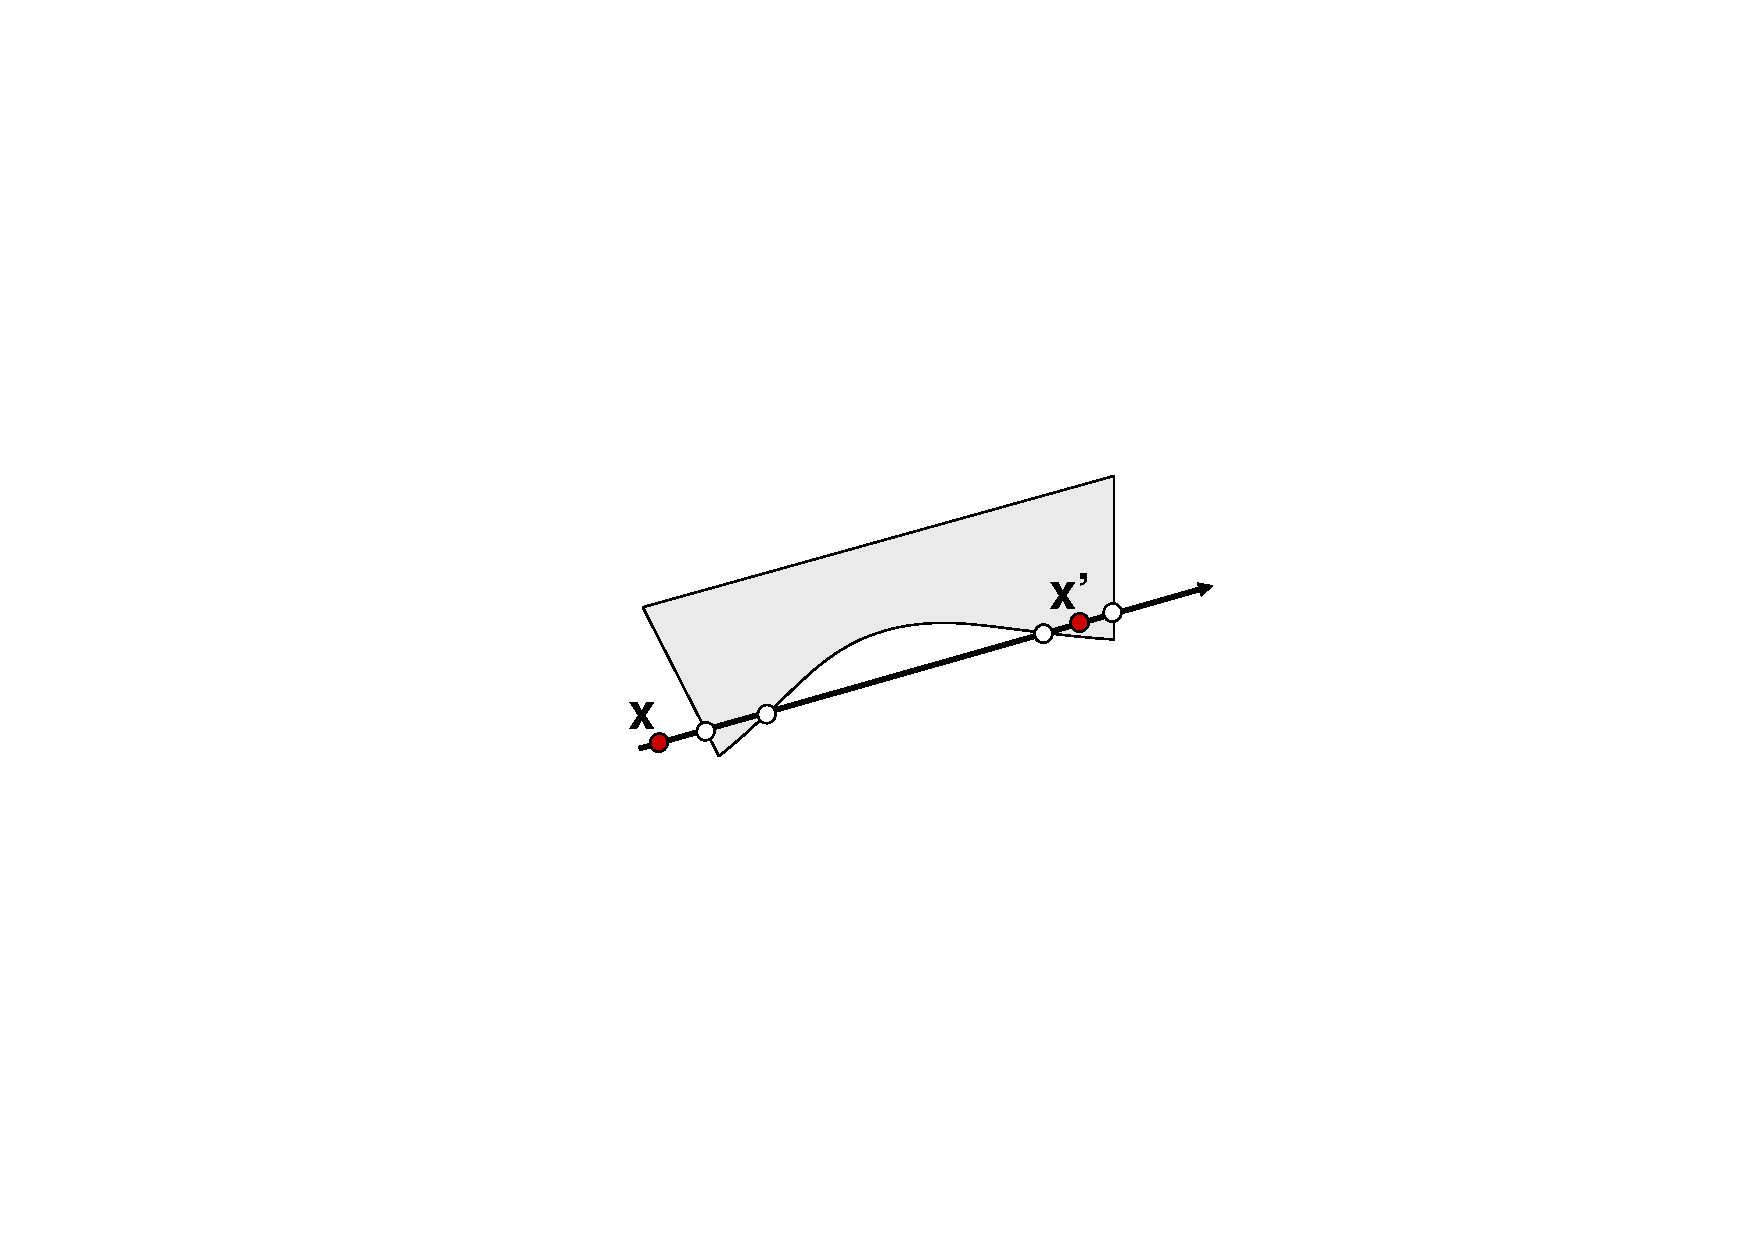
\includegraphics[width=0.8\textwidth]{img/05_stencil_walk_improved}
    \end{figure}
    Therefore \emph{exact} intersection points of the ray with bilinear surface patches must be calculated:
\end{itemize}

\paragraph{Exact intersection calculation} If the quadrangle is \emph{nonplanar} the four corners $P_0$, $P_1$, $P_2$, $P_3$ can be mapped to:
\begin{align*}
    \tilde P_0 &= (0,0,0)\\
    \tilde P_1 &= (1,0,0)\\
    \tilde P_2 &= (1,1,1)\\
    \tilde P_3 &= (0,1,0)
\end{align*}
by the \emph{affine transformation}
\begin{align*}
    \tilde x = (\tilde P_1 | \tilde P_2 | \tilde P_3) (P_1|P_2|P_3)^{-1} (x-P_0).
\end{align*}
The bilinear surface containing $P_0'$, $P_1'$, $P_2'$ and $P_3'$ is the \emph{hyperbolic paraboloid}
\begin{align*}
    z = xy.
\end{align*}
Inserting the transformed view ray $\tilde x + t\Delta \tilde x$ leads to a quadratic equation for $t$:
\begin{align*}
    (\tilde z + t\Delta \tilde z) = (\tilde x+t\Delta \tilde x)(\tilde y + t\Delta \tilde y).
\end{align*}
If real solutions with $0<t<1$ exist the intersection points $(\tilde x_i, \tilde y_i, \tilde z_i)$ are computed and transformed back.

In the second phase the stencil walk algorithm computes the local coordinates of the point in the cell known to contain it. The local coordinates are the inverse of the coordinate function:
\begin{align*}
    \phi: (\xi, \nu,\zeta)\mapsto (x,y,z)
\end{align*}
evaluate at the given point 
\begin{align*}
 x= (x,y,z).
\end{align*}
However, the trilinear function $\pi$ is a cubic polynomial and its inverse is a sixth-degree polynomial. Hence the problem needs to be solved with Newton's method.

\subsection{Global Point Location}
Global point location is more expensive than the stencil walk algorithm.

Many methods trade in safety for efficiency. A few methods are:
\begin{enumerate}
\item Search for the point in every grid cell using Newton's Method.

Hypothetic "brute force" method. Safe.
\item Buning's method.

Do incremental point location starting from a boundary cell. \textbf{Problem}:

Node $(O)$ nearest to given point $(X)$ is not necessarily adjacent to the cell containing it. Furthermore the straight line between the two points can leave the grid.
    \begin{figure}[H]
        \centering
        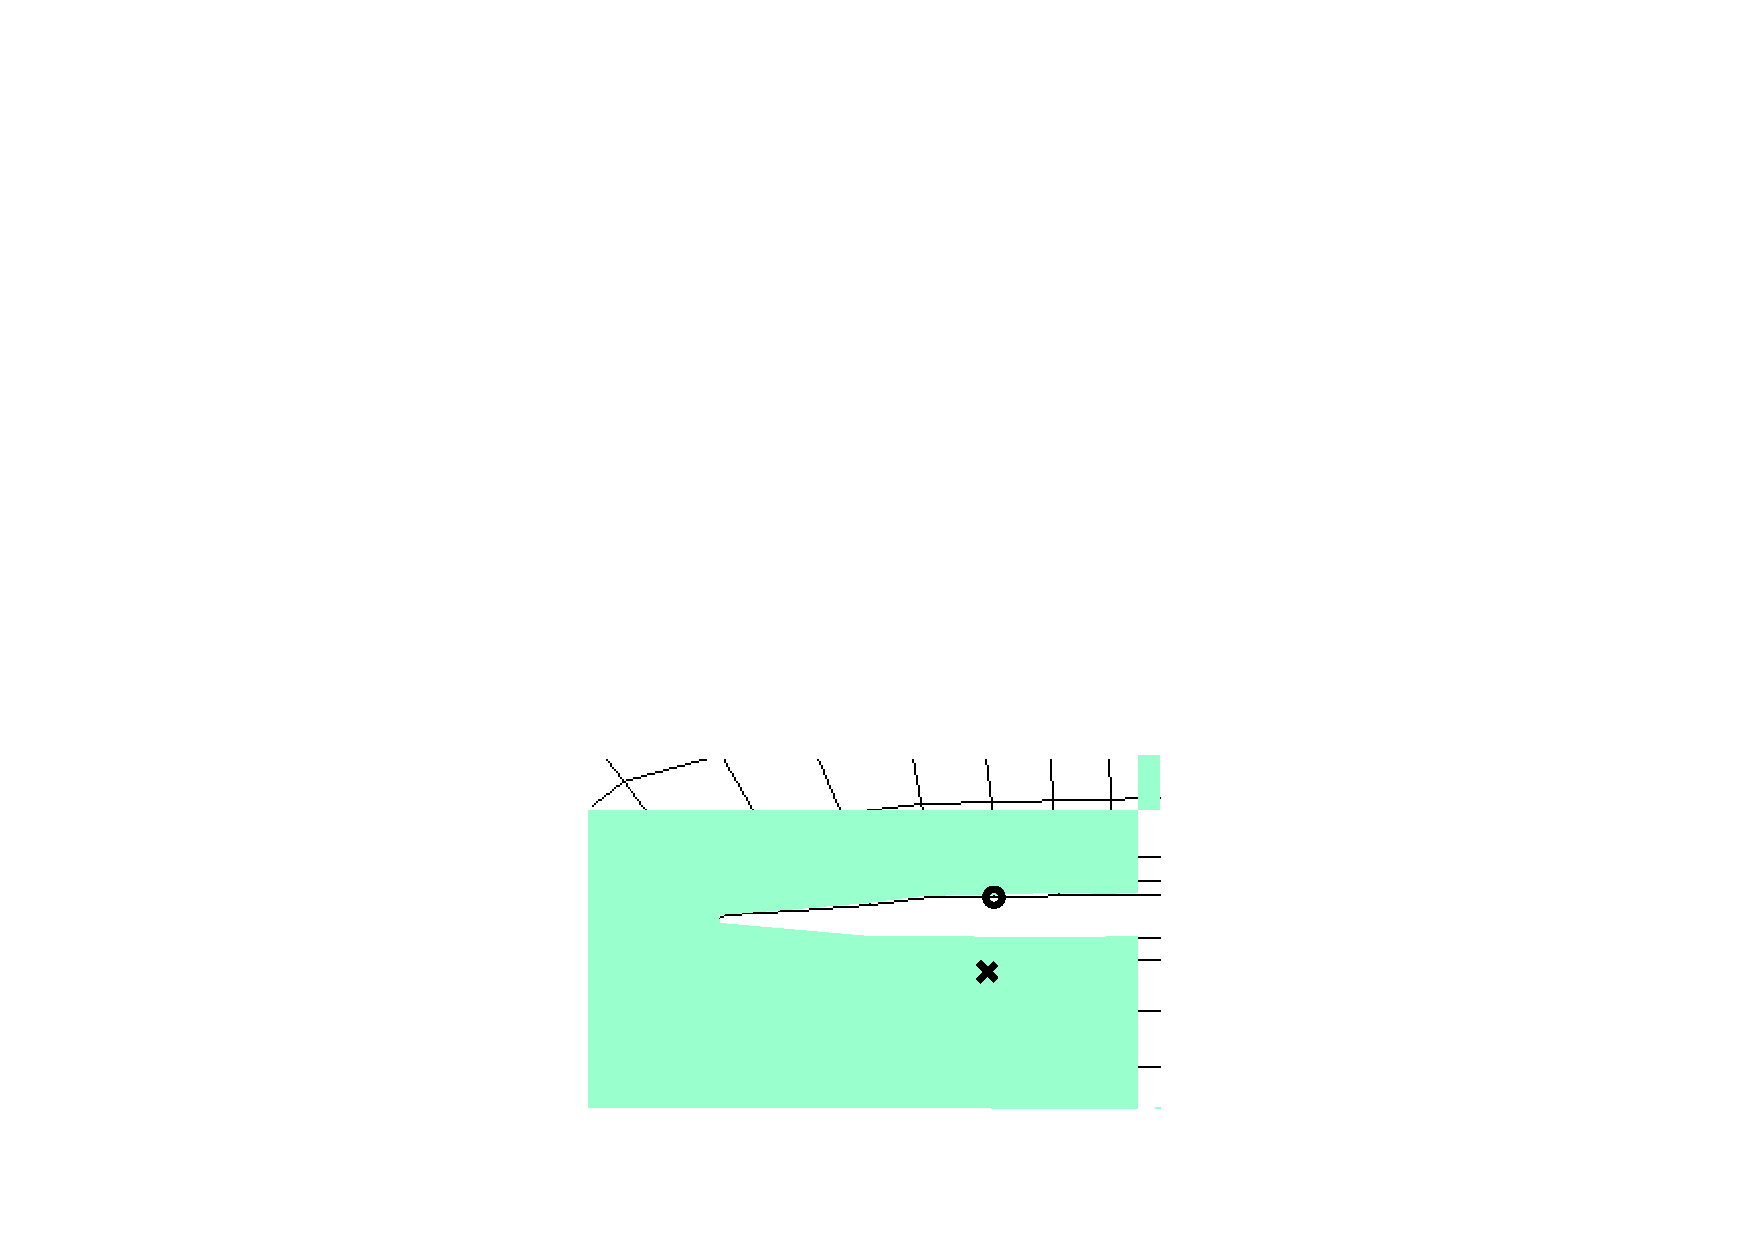
\includegraphics[width=0.5\textwidth]{img/05_bunings_method}
    \end{figure}
    
    Bunings method is safe if incremental search is repeated with a different boundary cell as long as the point is not found. Instead of using all boundary cells, precompute a subset of boundary cells to guarantee to find all points within the grid.
\item Incremental point location starting from a node near the grid center.

Simple method. Only safe for \emph{star-shaped} grids.
\item Search structure based.

Efficient methods use a search structure such as a uniform grid, octrees or kd-trees for nodes or cell centers:
\begin{itemize}
    \item When a point query is not sufficient a \emph{range query} is need with a range determined by the cell size.
    \item Problem: Cells can have extreme aspect ratios (especially from CFD).
\end{itemize}
\item Bounding box hierarchy

Use a bounding box hierarchy for a recursively subdivided grid. Efficient and safe method and easy for structured grids.

More preprocessing is required for unstructured grids (cell tree, Garth 2010)
\end{enumerate}

\subsection{Computational Space Streamline Integration}
In structured grids \emph{point location} can be \emph{avoided} by using a different approach:

Integration can be done in computational space $\mathcal C$ instead of physical space $\mathcal P$. This requires a modification of the integration algorithm:

\begin{itemize}
    \item \emph{Before} the integration step:
    
    Transform the \emph{velocity} $v(x)$ to $\mathcal C$ by multiplying with $J^{-1}$
    \item \emph{After} the integration step:
    
    This step is only required if graphical output of this step is needed. Transform the new \emph{position}
    \begin{align*}
         x= (i+\xi, j+\nu, k+\zeta)
    \end{align*}
    to $\mathcal P$ by trilinear interpolation.
\end{itemize}

Main problem of the integration in $\mathcal C$:
\begin{itemize}
    \item The ordinate function
    \begin{align*}
        \phi: (i+\xi,j+\nu, k+\zeta) \mapsto (x,y,z)
    \end{align*}
    is only $C^0$ continuous at cell boundaries.
    \item Therefore $J$ is discontinous.
    
    \item Example (Sadarjoen 1994): Four cells with a constant velocity field.
    \begin{figure}[H]
        \centering
        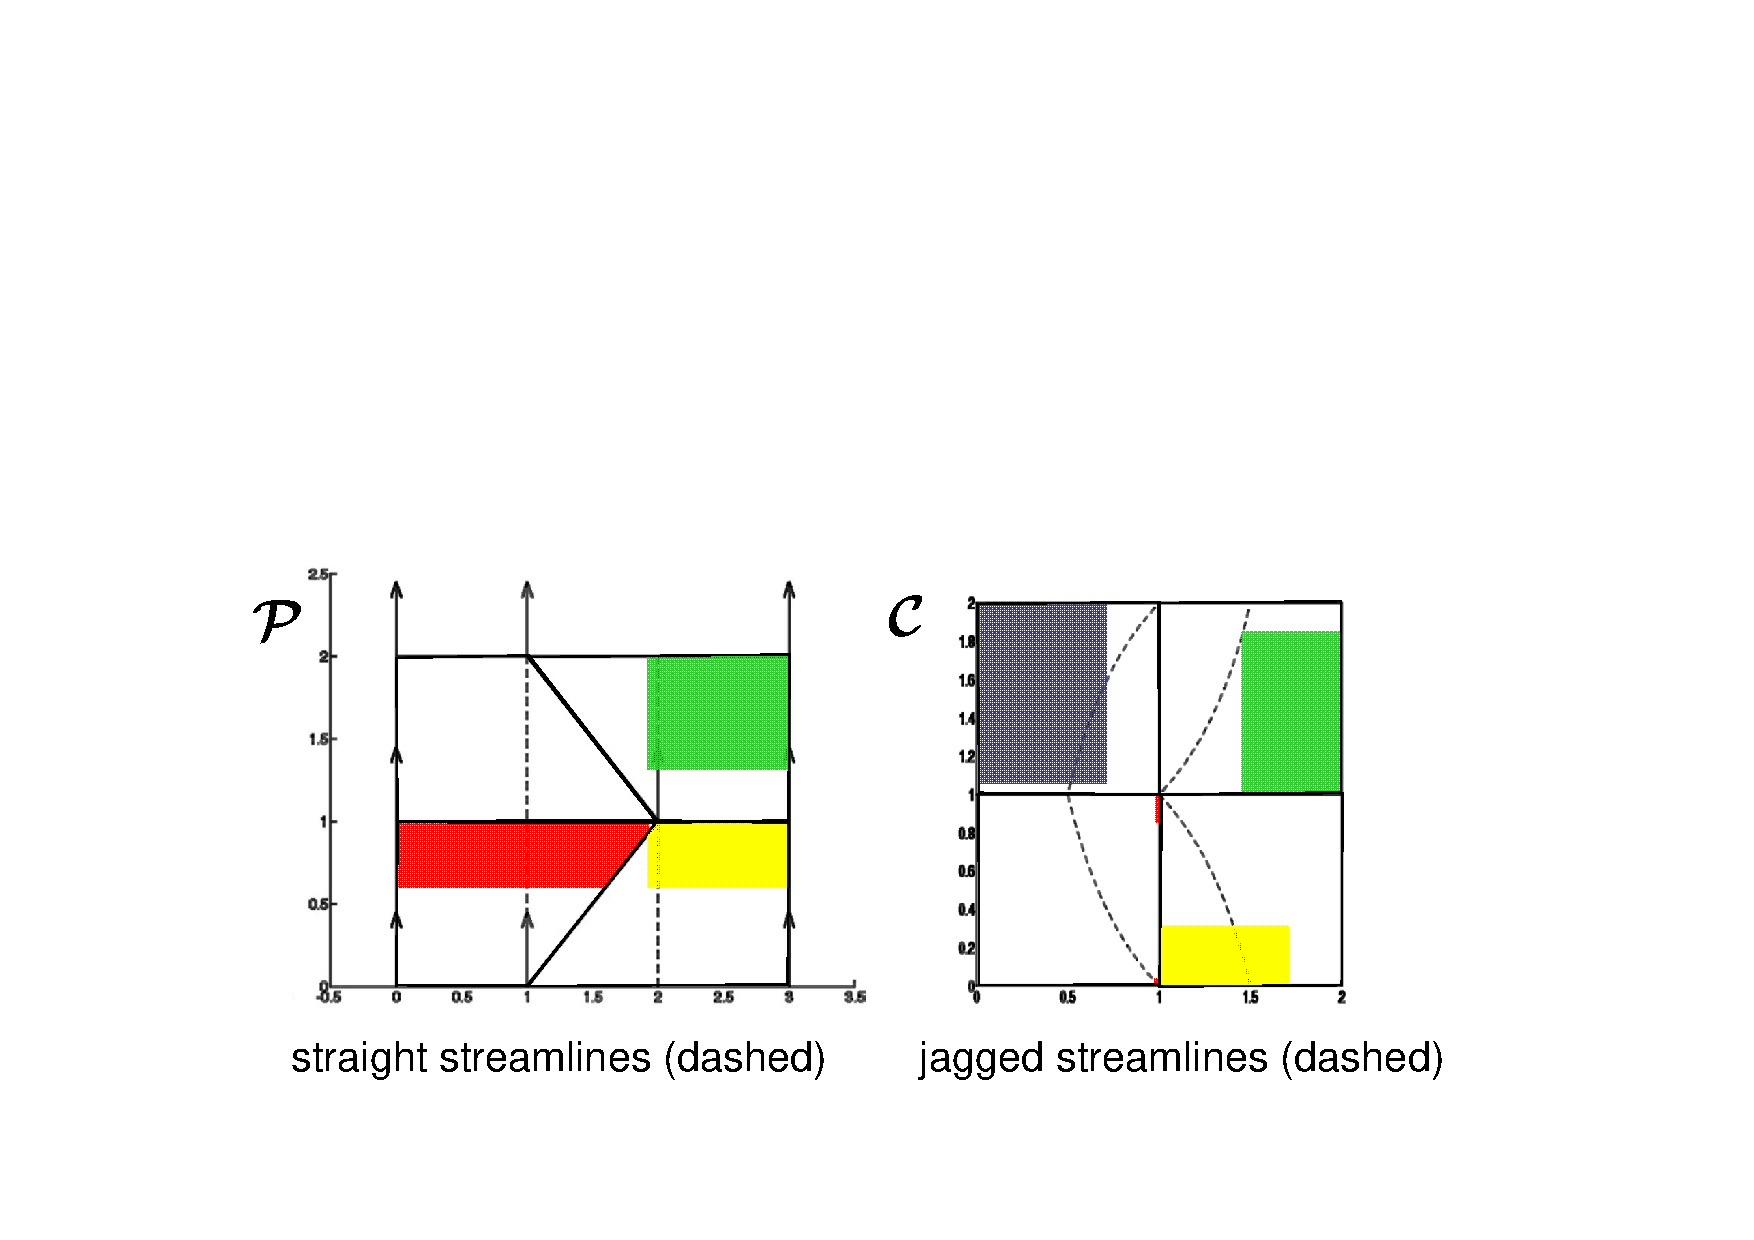
\includegraphics[width=0.6\textwidth]{img/05_cspace_integration_problem}
    \end{figure}
\end{itemize}

Two sources of error:
\begin{itemize}
    \item Integration steps across cell boundaries.
    
    This can be avoided by shortening such steps.
    
    \item Use of a (precomputed) single transformed field vector by node. 
    
    Can be fixed by transforming all eight vectors of a cell on the fly when entering a new cell.
\end{itemize}

The main advantage of integration in $\mathcal C$ is its algorithmic simplicity. But if it's done correctly (avoiding the errors above) it can be slower than an integration in $\mathcal P$.

\subsection{Skin Friction Lines}
Velocity fields of fluid flow can have grid boundaries which are walls (i.e. solid material surfaces). At walls the velocity vector is usually zero as a result of the no-slip boundary condition.
Therefore a derived vector field is often used: The \emph{wall shear stress}:
\begin{align*}
    \tau_w = \mu{\delta v_w\over \delta s},
\end{align*}
can be obtained as the limit of the wall-parallel velocity component $v_w$ divided by the wall distances $s$ and multiplied with the \emph{dynamic viscosity} $\mu$ (material constant). This limit is typically nonzero except at isolated points.

Streamlines of $\tau_w$ are called \emph{skin friction lines}. They are an example of a vector field defined on a surface in $3$-space.

\subsection{Streamline Placement}
The problems of visualisation by streamlines:
\begin{itemize}
    \item Dependency on seed points,
    \item and the density of streamlines can be largely inhomogogeneous.
\end{itemize}

\paragraph{Solution} Automatically optimise choice of seed points.
\begin{enumerate}
 \item \emph{Streamlets} (short streamline segments)
     
     The length is proportional to the velocity magnitude (obtained automatically by using a fixed integration time).
     
     Start with a uniform grid and make spacing roughy even by locally adapting (displacing, inserting, removing) seeds.

Typical use: Displaying weather maps

\item Algorithm by Turk and Bank (longer streamlines):

Objective: Create a streamline image which when low-pass filtered has a uniform grey level.

Optimise seed positions and integration lengths.

Operations:
\begin{itemize}
    \item Insert
    \item Delete
    \item Move
    \item Lengthen
    \item Shorten
\end{itemize}
Apply operations either randomly or based on oracles.

\end{enumerate}


\subsection{Streamsurfaces}
Definition: Union of streamlines seeded densly on a curve. 

Advantage for visualisation:
Structured, better spatial perception.

Naive algorithm:
\begin{itemize}
    \item Start integration at discrete samples on the seed curve.
    \item Conncect points of equal integration time resulting in a quad mesh.
\end{itemize}
This fails if streamlines diverge or grow at largely different speeds.
\begin{figure}[H]
    \centering
    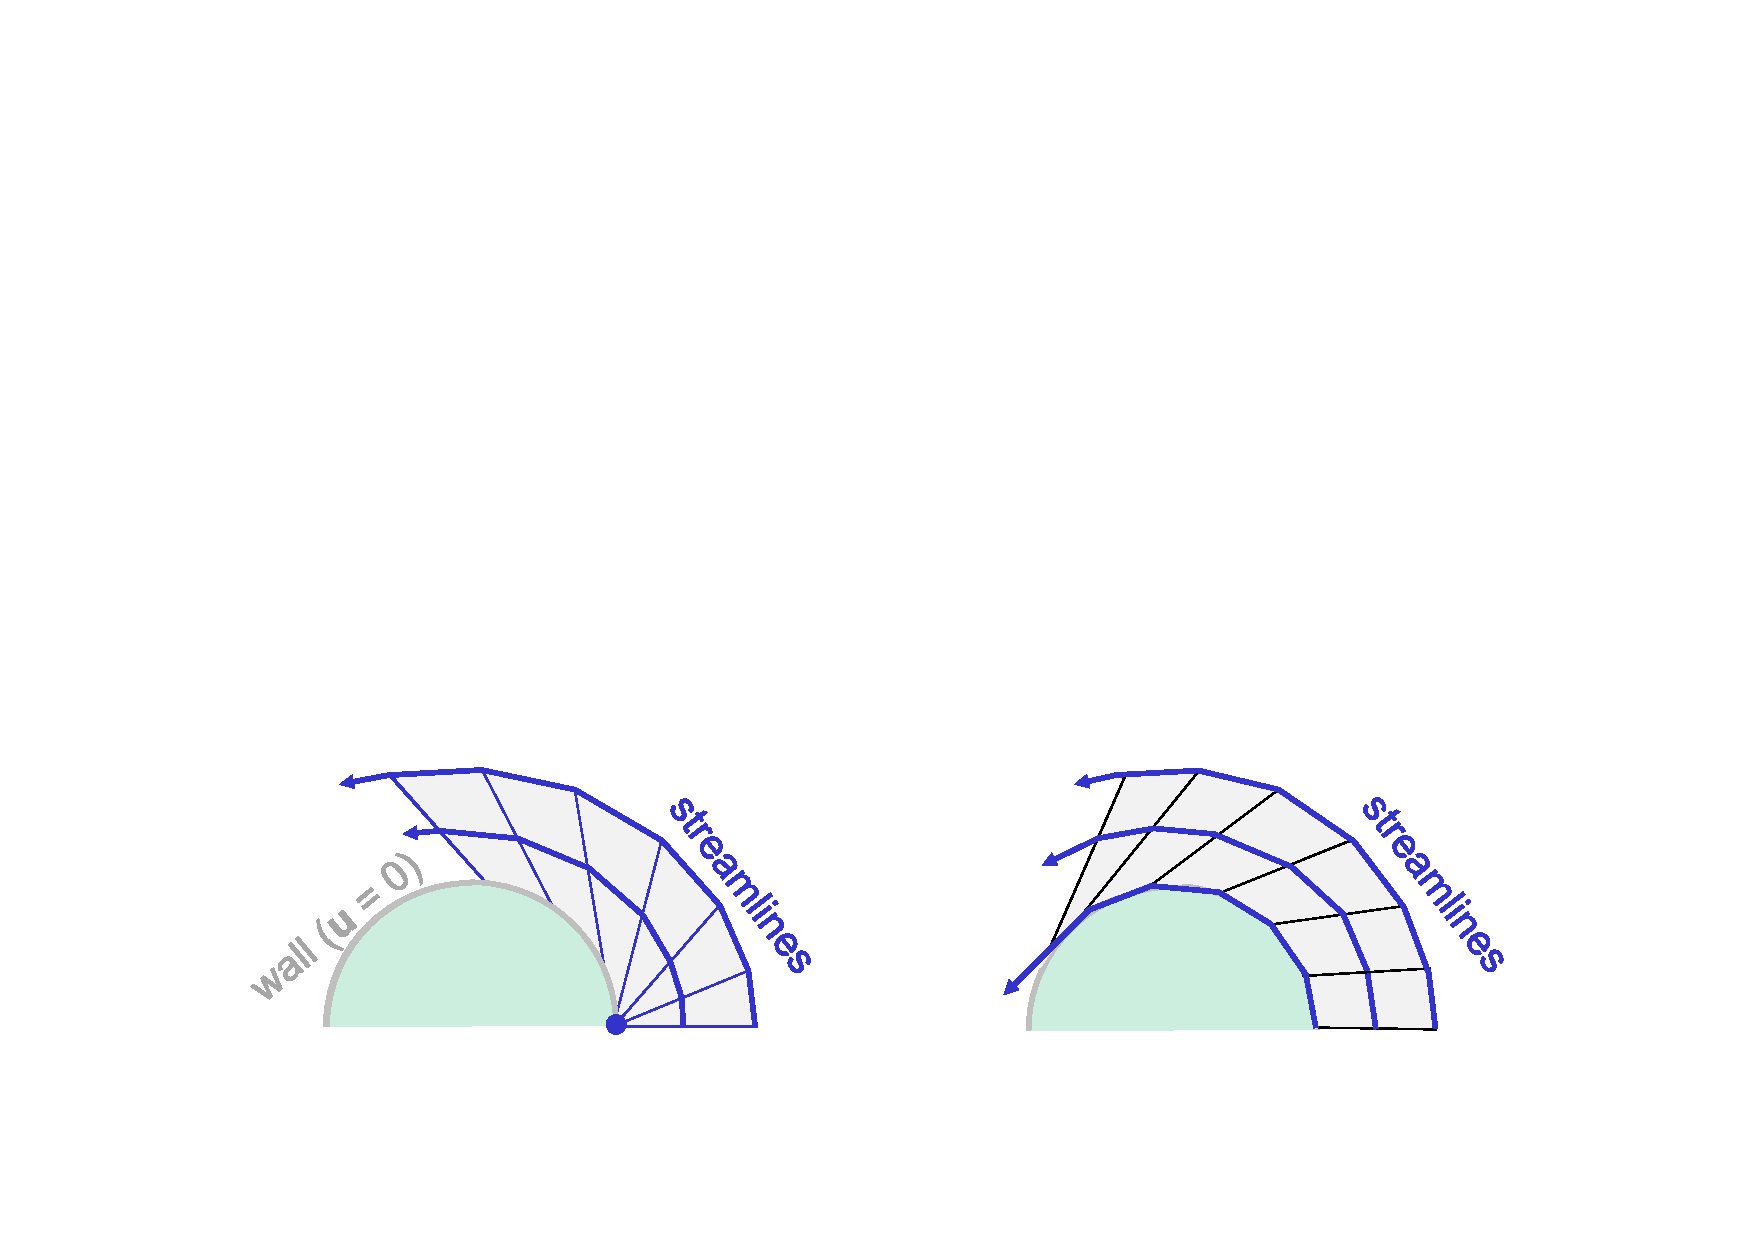
\includegraphics[width=0.8\textwidth]{img/05_streamsurfaces}
\end{figure}

\paragraph{Hultquist's algorithm} solves this problem of speed differences by \emph{optimised triangulation}: Of two possible connections choose the one which is closer to orthogonal (sic) to both streamlines.
\begin{figure}[H]
    \centering
    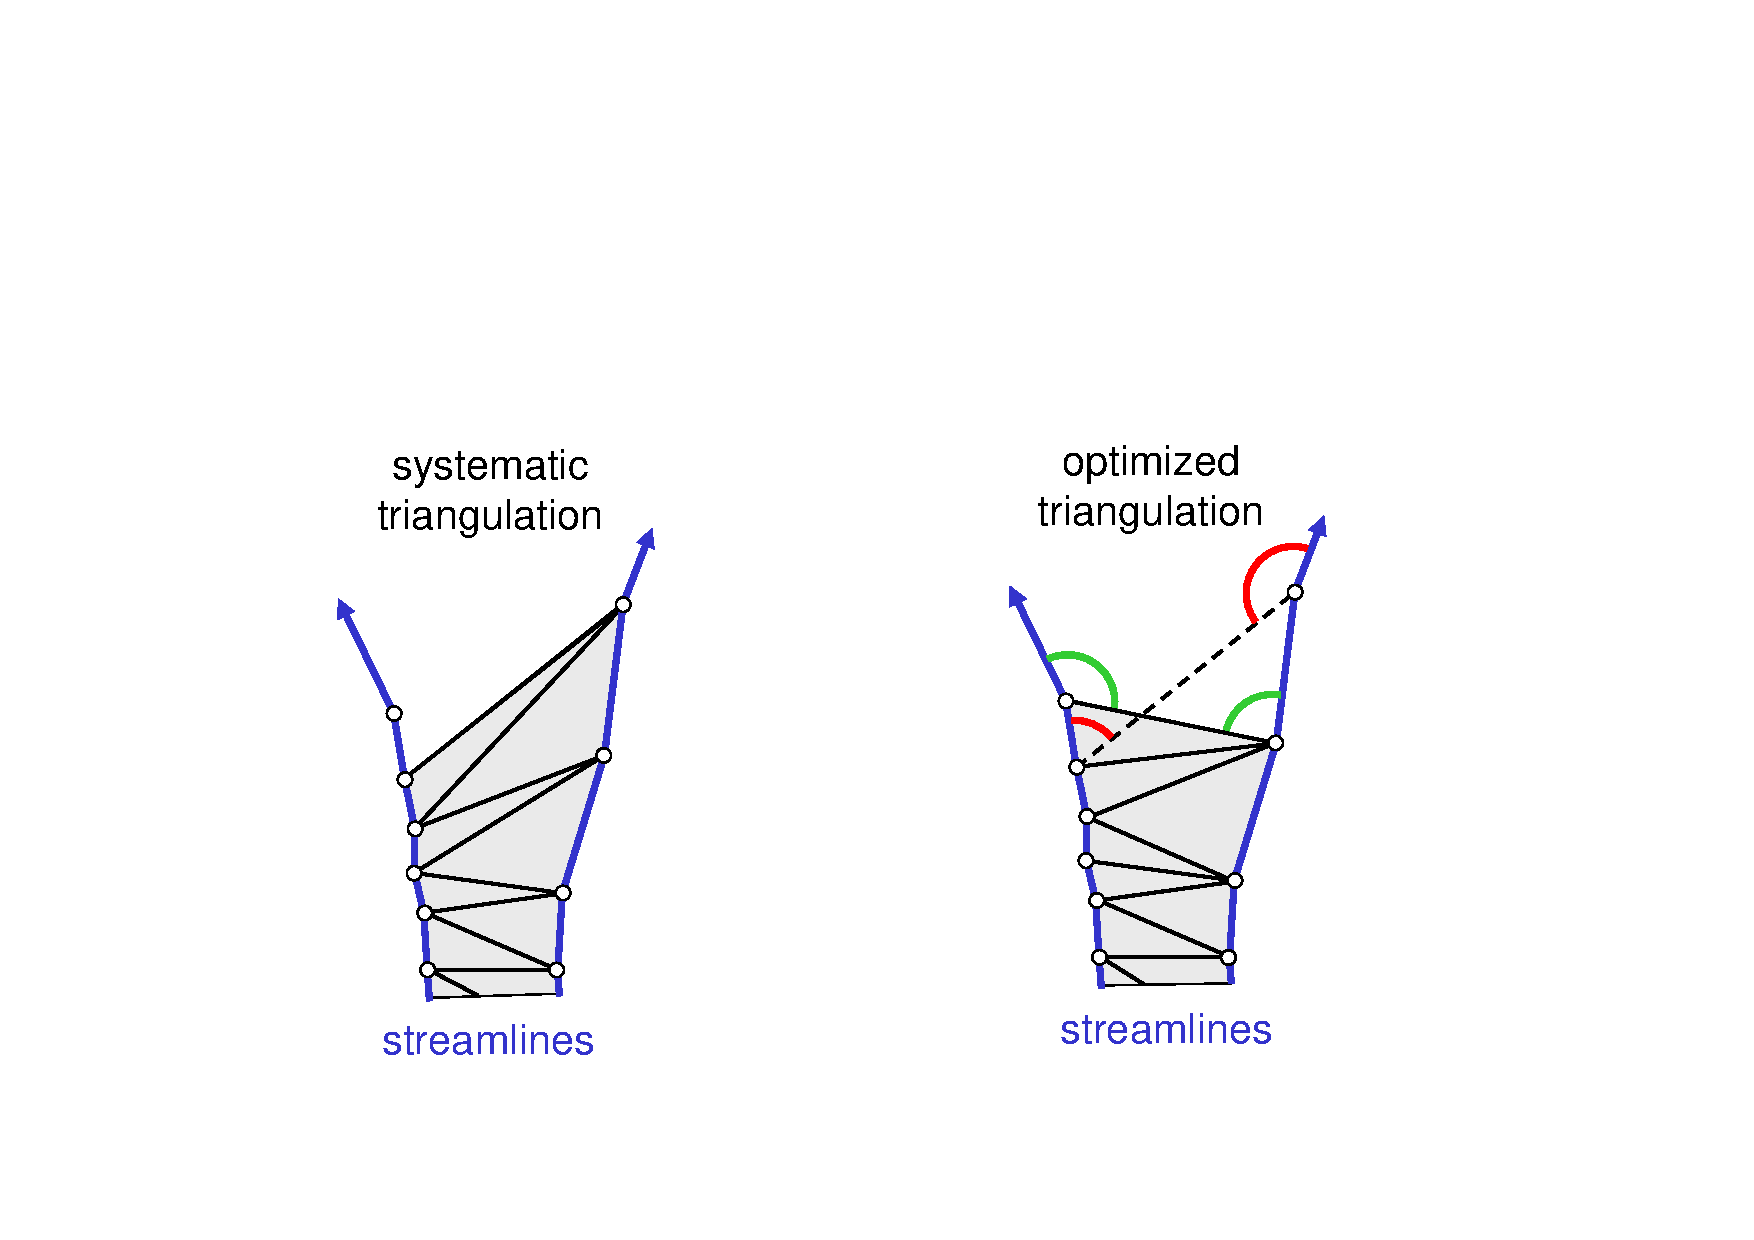
\includegraphics[width=0.8\textwidth]{img/05_hultquist}
\end{figure}
The problem of divergence or convergence is solved by \emph{inserting} or \emph{terminating streamlines}.
\begin{figure}[H]
    \centering
    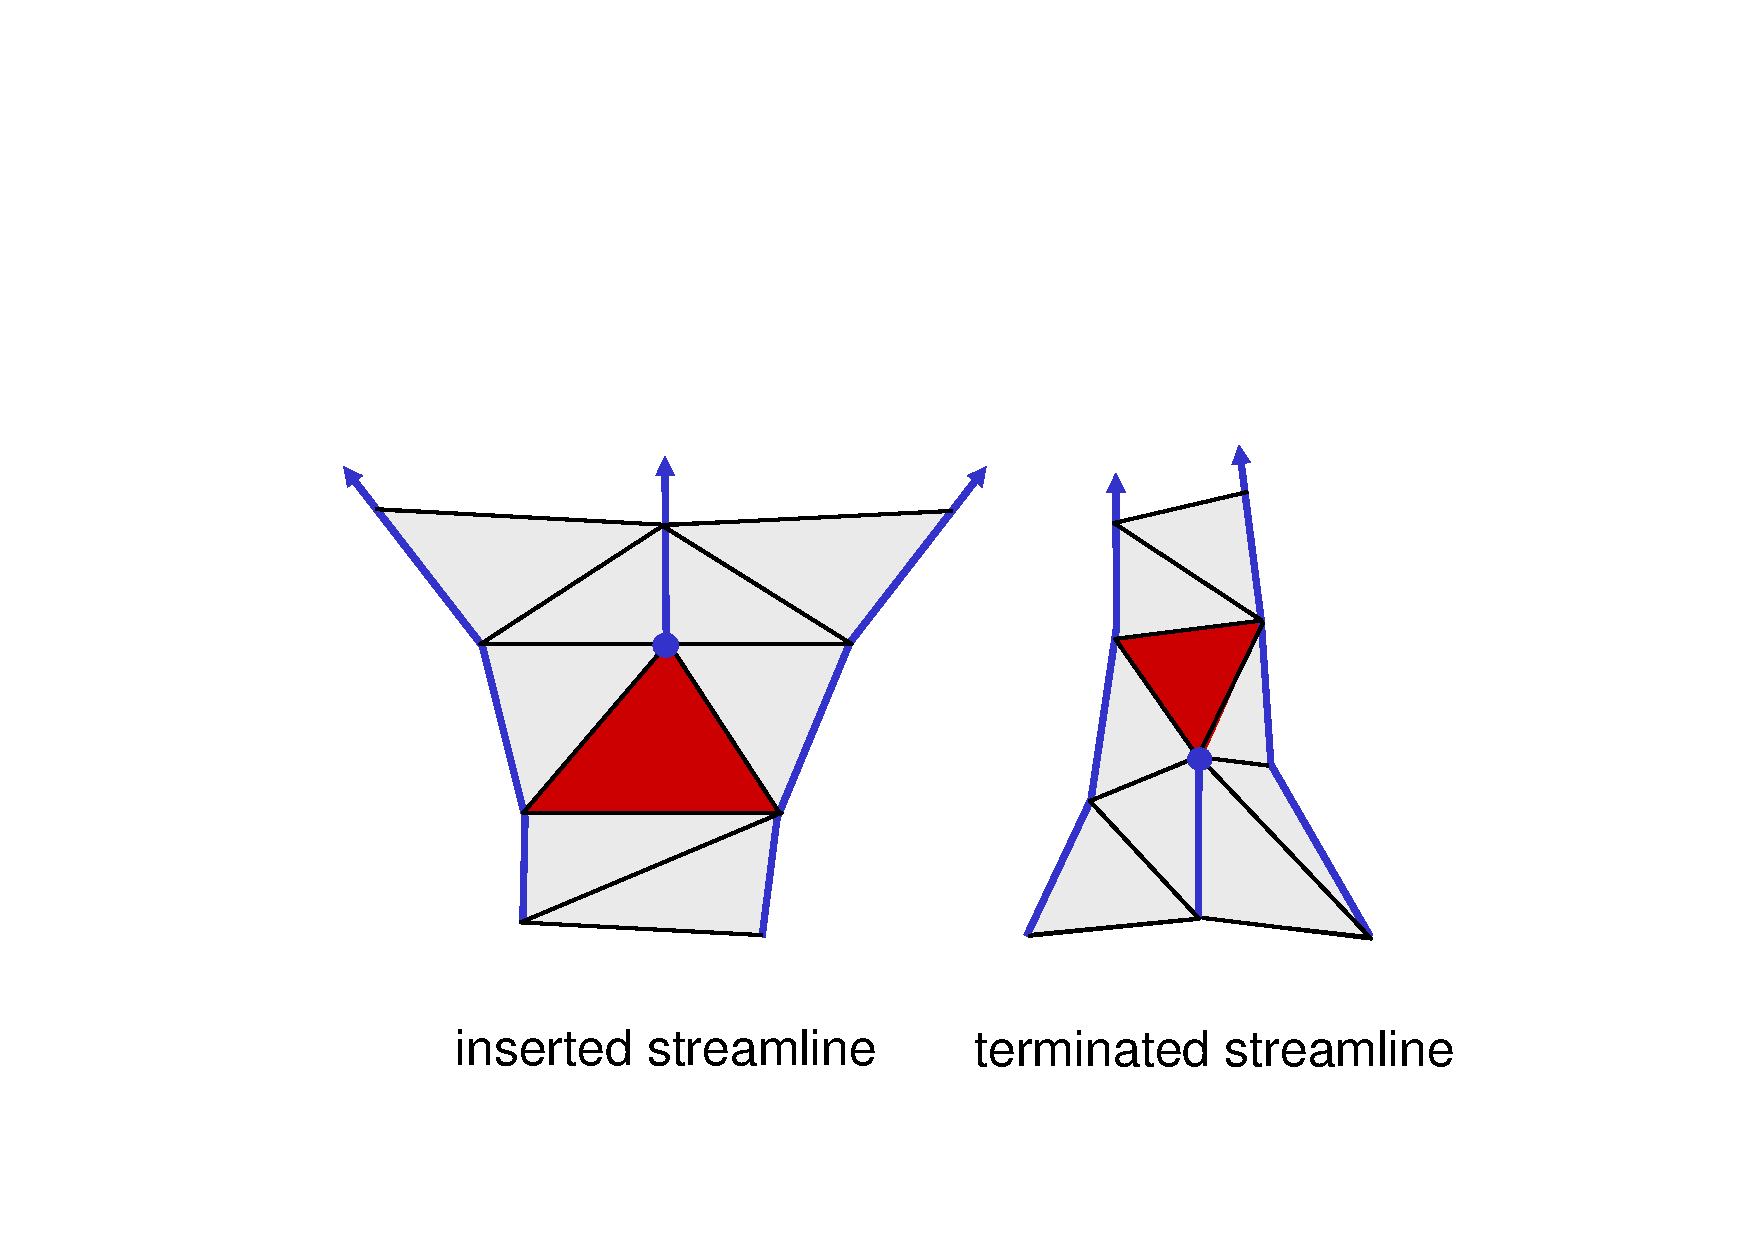
\includegraphics[width=0.8\textwidth]{img/05_hultquist_divergence}
\end{figure}

Also use hermite interpolation for streamsurface patches:
\begin{figure}[H]
    \centering
    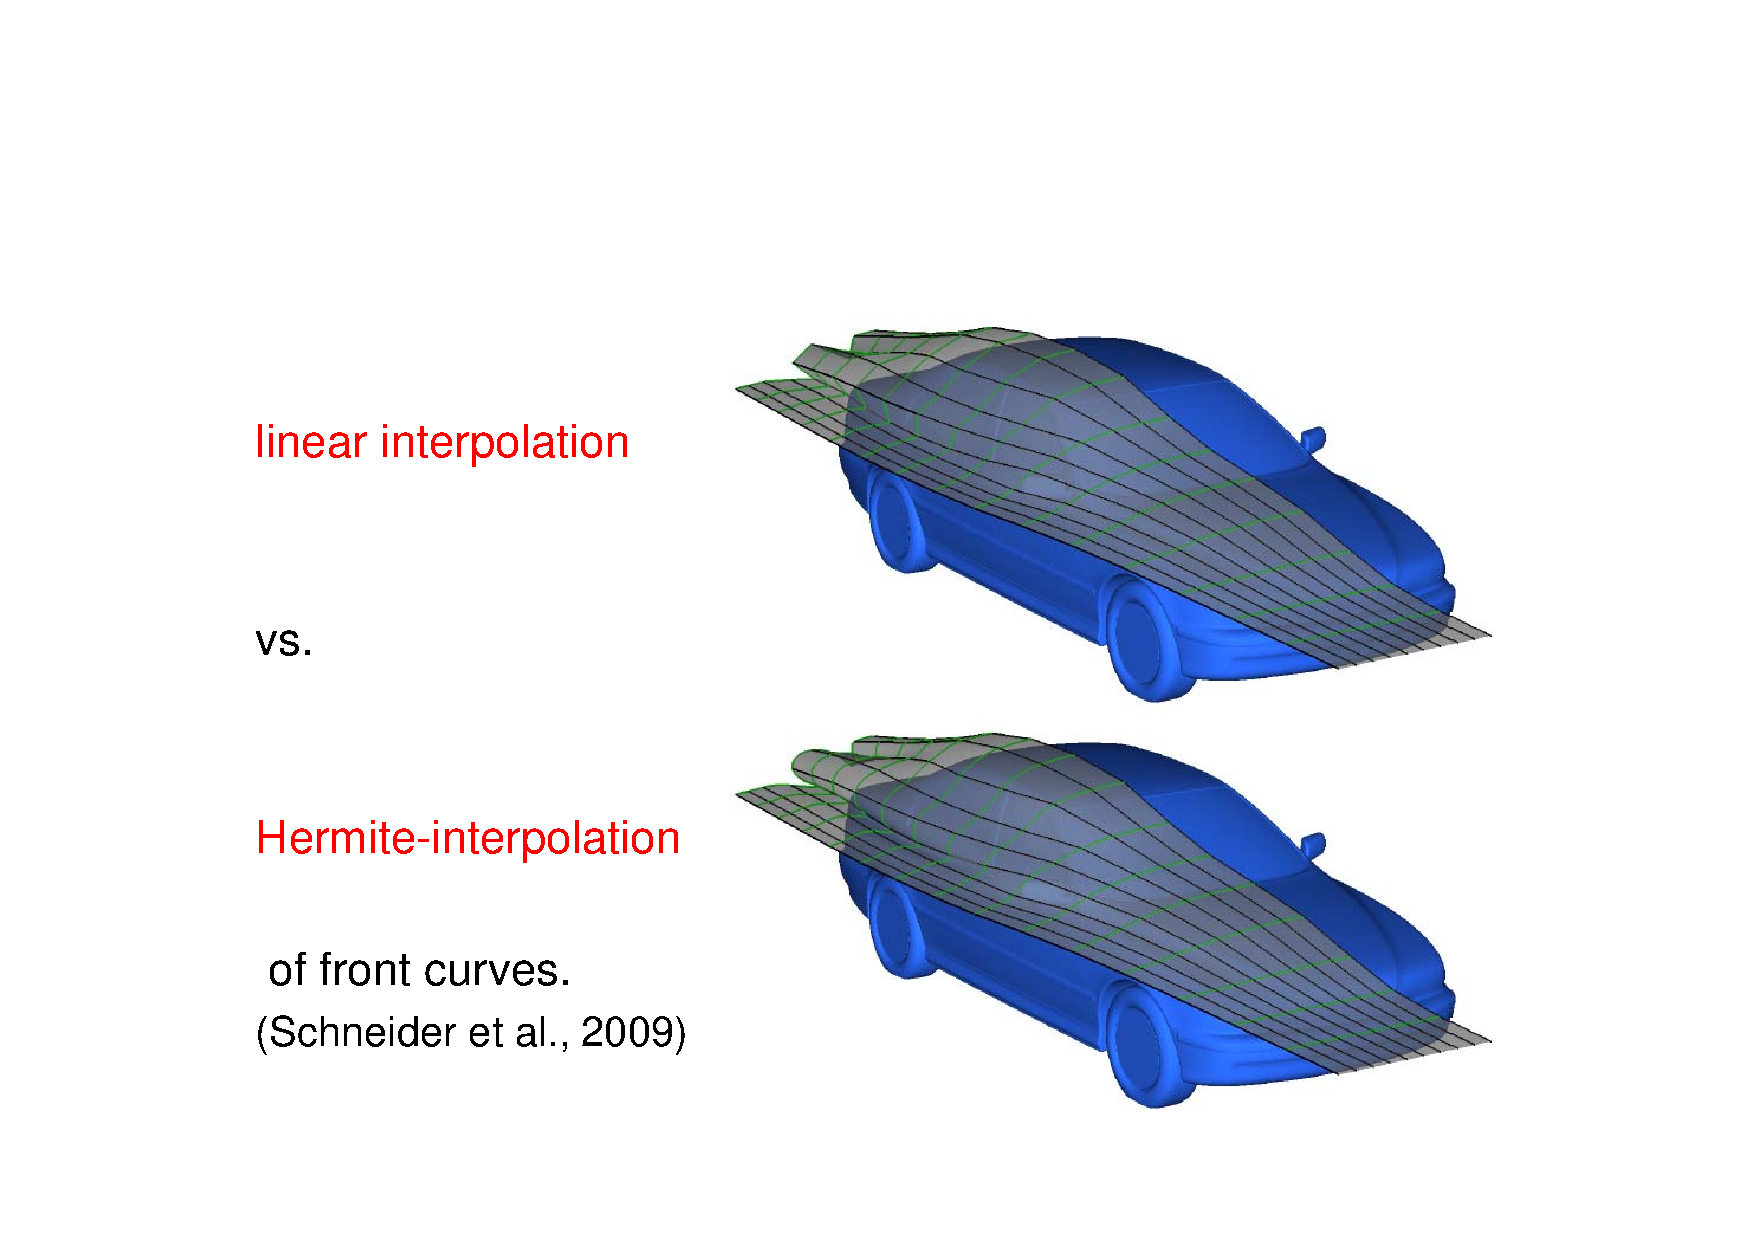
\includegraphics[width=0.8\textwidth]{img/05_hultquist_interpolation}
\end{figure}

\subsection{Streak Surfaces}
Stream lines in 3D on a fully adaptive triangle mesh.










